%The neurosciences, and more generally, brain and behavioral sciences, imply
%extensive interactions among disciplines to advance our 
%appreciation for the relation between brain and behavior. 
%\footnote{The Human Brain Project one such example.} 
%The inherent challenge, however, lies in bringing together the distributed competences
%of many individuals or even institutions and exchanging across interdisciplinary
%borders using common techniques.  
%This situation is excerbated by the technical sophistication of modern
%data analysis and brain simulation, which often impedes their adoption 
%in the communtiy.
%
Neuroscience has evolved through extensive interactions among disciplines
to advance our appreciation of the relation between brain and behavior.
The interdisciplinary nature of the field presents formidable challenges
for effective collaboration.

These challenges call for two kinds of solutions. First, there is a need
for comprehensive, modern computational libraries written in a widely
used and available programming languages; current examples include MNE-Python \citep{mnepython},
a Python package for treating M/EEG data via time-frequency analyses and inverse
solutions and the Brain Connectivity
Toolbox \citep{rubinov2010complex} for analyzing the graph theoretic
properties of structural and functional connectivity. Second, there is
a need for the implementation
of collaborative infrastructure for sharing not only data, but expertise; 
CARMEN \citep{austin2011carmen} and G-Node \citep{herz2008g} are two such
examples of developing platforms for collaborative work and data sharing, 
in the domains of cellular and systems neurophysiology.

TheVirtualBrain (TVB)
provides new tools to facilitate the collaboration between experimentalists and modelers by
exposing both a comprehensive simulator for brain dynamics and an integrative 
framework for the management, analysis simulation of structural and functional
data in an accessible, web-based interface. The choice of Python was made based on
its wide use as the high-level language in scientific programming, 
the unparalleled open-source libraries and tools available, and strong software engineering 
culture.
This choice was confirmed by the publication of the first issue of Python 
in Neuroscience and has made it possible for the entirety of TVB from the 
numerical algorithms to the web server to be written in Python.

\subsection{The framework}

 \begin{figure*}
        \centering
        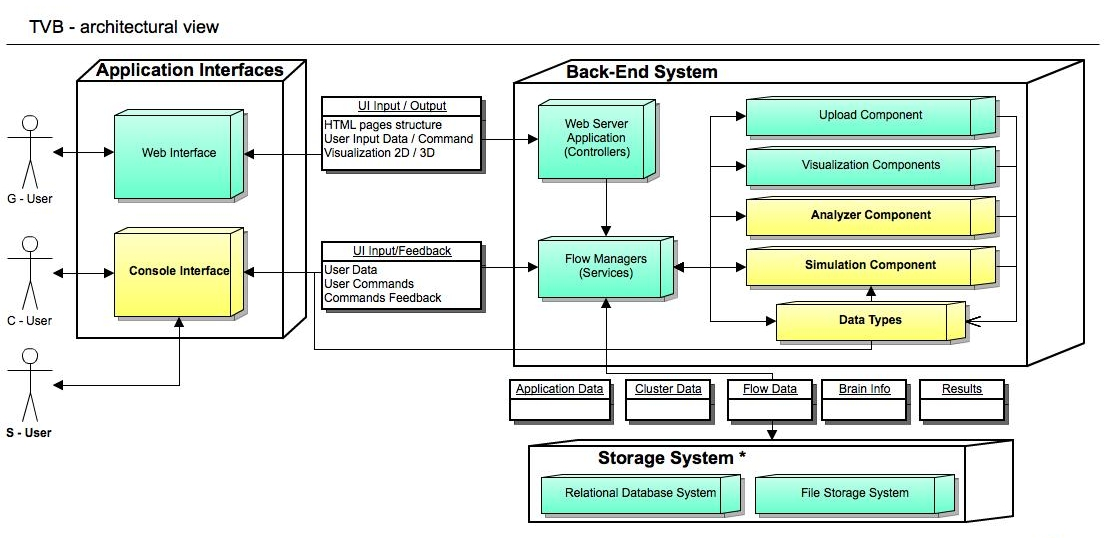
\includegraphics[width=0.90\textwidth]{images/architecture.jpg}
        \caption{TVB architecture: Yellow blocks are part of the scientific
            library of TVB, while the green blocks are part of TVB Framework.
            TVB provides two independent interfaces, depending on the
            interaction type desired the end-user (web or console).  TVB
            Storage layer is compulsory for the web interface, but it can be
	    switched on/off for the console interface.  The terms \textit{G-User},
	    \textit{C-User} and \textit{S-User} refer to users of the graphical,
	    console \& database and scripting components. Here, console interface
	    is conceptual and refers only to existing Python command lines, IPython
	    included. 
         }
        \label{fig:architecture}
 \end{figure*}

The TVB framework was developed to allow easy integration of any
computational tools along with a system for describing typical types of data.
Additionally, 
two main constraints for the framework were to provide a web
interface to allow remote collaboration and the
exchange of data (or simulation results) between users, especially for
users not comfortable programming. The web interface
and database backend are built on combination of 
the \textsf{CherryPy} and \textsf{SQLAlchemy} packages.
\footnote{The full list of dependencies can be found in the
project's documentation.}
The overall structure of TVB is depicted in Figure~\ref{fig:architecture}.

\subsection{The simulator}

A significant part of TVB is simulating large-scale brain networks. While
several existing simulators could have been adapted, we have estimated that
TVB style simulations are far enough outside the design of other simulators to
make a new development necessary. We discuss these reasons in the following. 

Existing neural network simulators typically focus either on abstract rate neurons, 
modelling  neurocognitive processes, or 
full multicompartmental neurons treating complex spatial
geometries, e.g. NEURON \citep{Hines_2001}, modelling the interaction of 
channel distributions in dendrites.  More recently, due to interest in
the computational properties of spiking neurons and their relevance to
experimental observations, simulators designed for spiking or oscillating neurons
have become prominent, including Brian \citep{Goodman_2009}, which we initially 
considered for our simulations.
In TVB the network is defined with neural mass or field
models \citep{Deco_2008a, Coombes_2010} rather than cellular models. The
spatial extent of the modeled dynamics is macroscopic and scales reasonably 
to the entire cortex, and uses empirical measurements of corticocortical
connectivity. Several technical issues are unique to this scale, such
as efficient handling of dense $N^2$ inter-regional delays and integration
of neural field-like models and connectivity on triangular meshes in 3D.
Finally, comparison with experimental data requires forward solutions
that transform physiological signals to the commonly
used imaging modalities such as EEG, MEG and fMRI need to be employed.
For these reasons, TVB required a new simulator, built around the paradigm
of whole-brain scale simulation.

\subsection{Obtaining and contributing to TVB}

The easiest way to get started with TVB is to download a distribution
from \url{http://www.thevirtualbrain.org}, which is available for Windows,
Mac OS X and Linux. This distribution includes
all of pieces, from the simulator to the web interface, and has no
requirements other than a modern web browser supporting WebGL, SVG and
HTML5.

Alternatively, because TVB is licensed under the GPL, the sources may be
readily obtained from the public Git repositories hosted on Github
\citep{dabbish2012social}, at 
\url{https://github.com/the-virtual-brain}. In order to use the simulator, 
only the standard scientific Python packages are required (NumPy \& SciPy).
The framework and web interface depend on a few more packages. 

We provide an API doc, built from the docs strings using Sphinx.
User's, Contributor's and Developer's manuals are also provided with TVB
distributions in PDF format. The source files (in .rst) are available
through the Github repository \url{https://github.com/the-virtual-brain/docs}.  
In addition, IPython notebooks \citep{PerezGranger_2007}
for interactive tutorials are provided. These are based on the
demonstration scripts provided with the scientific library, and
include a more detailed description of the scientific goal (if
applicable), the components and stages of a simulation as well as a
brief description in the case of reproducing previous work. Users
interacting with \TVB GUI may also benefit from these tutorials
(\url{https://github.com/the-virtual-
brain/scientific_library/wiki/Tutorials}) when displayed as snippets
with IPython nbviewer. 

Additionally, the user interface provides an online help overlay, that pulls
information from the User's manual.


